% Jurnal RESTI (Rekayasa Sistem dan Teknologi Informasi)
% Template: IAII RESTI Format (Times New Roman, 1.5 spacing, A4)
% Compile: lualatex resti_paper.tex (or xelatex for TTF fonts)

\documentclass[a4paper,12pt]{article}

\usepackage[utf8]{inputenc}
\usepackage[english,bahasa]{babel}
\usepackage{times}
\usepackage{graphicx}
\usepackage{amsmath,amssymb}
\usepackage{booktabs}
\usepackage{hyperref}
\usepackage[numbers]{natbib}
\usepackage{setspace}
\usepackage{geometry}
\usepackage{indentfirst}
\usepackage{caption}
\usepackage{algorithm}
\usepackage{algpseudocode}
\usepackage{float}
\usepackage[table]{xcolor}

\geometry{left=2.5cm,right=2.5cm,top=2.5cm,bottom=2.5cm}

\onehalfspacing
\setlength{\parindent}{1.5em}

\hypersetup{colorlinks=true,linkcolor=black,urlcolor=blue,citecolor=black}

\renewcommand{\captionfont}{\footnotesize}
\renewcommand{\captionlabelfont}{\bfseries\footnotesize}

\begin{document}

\title{\textbf{Automasi Web Penetration Testing Menggunakan\\Reinforcement Learning: Studi Komparatif Q-Learning,\\Deep Q-Network, dan OWASP ZAP}}
\author{%
  Kevin Setiawan\textsuperscript{1,*}, Advisor Name\textsuperscript{1}\\
  \textsuperscript{1}Program Studi Informatika, Universitas Contoh, Indonesia\\
  \textsuperscript{*}Email: kevin.setiawan@example.com
}
\date{}
\maketitle

% ===================================================================
\begin{abstract}
Web application security testing is a critical yet resource-intensive aspect of modern cybersecurity. This paper investigates reinforcement learning (RL) for automated web penetration testing through a comparative study of tabular Q-Learning and Deep Q-Network (DQN) agents on OWASP Juice Shop. We formulate penetration testing as a Markov decision process with an 8-dimensional state space and a composite action space of 88 discrete actions combining 11 attack payloads across 8 endpoints (5 GET, 3 POST). A false-positive verification mechanism using benign probes is introduced to improve detection precision. Experimental results over 200 episodes demonstrate that Q-Learning with optimistic initialization achieves a 91.5\% detection rate (183 vulnerabilities, 1.09 requests/vulnerability), significantly outperforming DQN (61.5\%, 1.63 req/vuln) and OWASP ZAP (0.13\%, 792.5 req/vuln) on identical endpoints. Our approach demonstrates a 727-fold improvement in requests per vulnerability over the industry-standard scanner, establishing that tabular Q-Learning offers the best balance of efficiency, accuracy, and simplicity for small-to-medium scale web penetration testing.
\end{abstract}

\begin{center}
\rule{0.8\textwidth}{0.5pt}
\end{center}

\section*{Abstrak}
Pengujian keamanan aplikasi web merupakan aspek kritis dalam keamanan siber modern yang membutuhkan sumber daya dan keahlian signifikan. Penelitian ini menginvestigasi penggunaan \textit{reinforcement learning} (RL) untuk mengotomasi \textit{web penetration testing} melalui studi komparatif antara Q-Learning tabular dan Deep Q-Network (DQN) pada platform OWASP Juice Shop. Permasalahan pengujian penetrasi diformulasikan sebagai \textit{Markov decision process} dengan representasi \textit{state} 8 dimensi yang menangkap kode status HTTP, panjang respons, \textit{error flag}, pantulan \textit{payload}, indeks \textit{endpoint}, waktu respons, dan tipe konten, serta \textit{action space} komposit sebanyak 88 aksi diskrit yang mengombinasikan 11 \textit{payload} serangan pada 8 \textit{endpoint} (5 GET, 3 POST). Mekanisme verifikasi \textit{false positive} menggunakan \textit{probe} benign diperkenalkan untuk meningkatkan presisi deteksi. Hasil eksperimen pada 200 episode menunjukkan bahwa Q-Learning dengan \textit{optimistic initialization} mencapai tingkat deteksi 91,5\% (183 kerentanan, 1,09 permintaan per kerentanan), melampaui DQN (61,5\%, 1,63 req/vuln) dan OWASP ZAP (0,13\%, 792,5 req/vuln) pada \textit{endpoint} yang identik. Q-Learning berhasil mengidentifikasi 173 SQL \textit{injection}, 6 \textit{reflected} XSS, dan 4 anomali \textit{fuzzing}. Pendekatan ini menunjukkan peningkatan efisiensi 727 kali lipat dalam jumlah permintaan per kerentanan dibandingkan \textit{scanner} industri standar, mengonfirmasi bahwa Q-Learning tabular menawarkan keseimbangan terbaik antara efisiensi, akurasi, dan kesederhanaan untuk pengujian penetrasi web skala kecil hingga menengah.

\medskip
\noindent\textbf{Kata kunci:} \textit{reinforcement learning}, Q-learning, \textit{deep Q-network}, \textit{penetration testing}, keamanan web, OWASP Juice Shop, deteksi kerentanan otomatis

\begin{center}
\rule{0.8\textwidth}{0.5pt}
\end{center}

% ===================================================================
\section{Pendahuluan}
% ===================================================================

Aplikasi web tetap menjadi permukaan serangan utama dalam keamanan siber modern. SQL \textit{injection} (SQLi), \textit{cross-site scripting} (XSS), dan \textit{path traversal} secara konsisten menempati peringkat teratas dalam OWASP Top Ten \cite{owasp2021}. \textit{Penetration testing} -- simulasi serangan untuk mengidentifikasi dan mengeksploitasi kelemahan keamanan sebelum pelaku kejahatan melakukannya -- merupakan praktik pertahanan esensial. Namun, pengujian penetrasi konvensional bersifat padat karya, bergantung pada keahlian, dan sulit diskalakan \cite{holm2017}.

Pemindai kerentanan otomatis seperti OWASP ZAP \cite{zap2024} dan Burp Suite \cite{burpsuite} mengatasi masalah skalabilitas tetapi mengikuti pendekatan statis berbasis aturan. Setiap pemindaian mengeksekusi serangkaian \textit{probe} tetap tanpa mempertimbangkan hasil sebelumnya, menghasilkan ratusan permintaan redundan per kerentanan yang ditemukan. Kurangnya adaptivitas ini membuat pemindai tradisional sangat tidak efisien untuk pengujian berkelanjutan dalam \textit{pipeline} CI/CD, di mana \textit{feedback} yang cepat dan terarah sangat penting.

\textit{Reinforcement learning} (RL) menawarkan alternatif yang menjanjikan: agen RL belajar strategi serangan optimal melalui interaksi coba-coba, secara dinamis menyesuaikan pemilihan \textit{payload} dan penargetan \textit{endpoint} berdasarkan respons yang diamati \cite{erdodi2022,zhou2021autonomous}. Dengan memformulasikan pengujian penetrasi sebagai pengambilan keputusan sekuensial, agen berbasis RL berpotensi meningkatkan efisiensi deteksi secara dramatis.

Penerapan RL pada \textit{penetration testing} telah menghasilkan temuan menjanjikan di lingkungan jaringan simulasi \cite{becker2024,ghanem2020,venturi2024}. Namun, beberapa kesenjangan masih ada. Sebagian besar studi mengevaluasi pada simulator jaringan daripada aplikasi web nyata, menggunakan \textit{action space} yang tidak bergantung pada \textit{endpoint}, dan tidak melakukan perbandingan terkontrol dengan pemindai kerentanan standar pada \textit{endpoint} yang identik.

Penelitian ini bertujuan mengisi kesenjangan tersebut melalui kontribusi sebagai berikut:
\begin{enumerate}
  \item Representasi \textit{state} 8 dimensi dan \textit{action space} komposit (11 \textit{payload} $\times$ 8 \textit{endpoint} = 88 aksi) yang memungkinkan pembelajaran kebijakan sadar-\textit{endpoint}, dengan dukungan untuk \textit{endpoint} GET dan POST.
  \item Evaluasi komparatif antara Q-Learning tabular (dengan \textit{optimistic initialization}) dan DQN pada kondisi eksperimental yang identik di OWASP Juice Shop, termasuk mekanisme verifikasi \textit{false positive}.
  \item Perbandingan terkontrol dengan OWASP ZAP pada \textit{endpoint} identik yang mengukur keunggulan efisiensi 727$\times$ dalam jumlah permintaan per kerentanan.
  \item Kerangka kerja eksperimental yang \textit{reproducible} dengan konfigurasi hiperparameter terperinci, \textit{pseudocode} algoritma, dan implementasi \textit{open-source}.
\end{enumerate}

Sisa artikel ini diorganisasikan sebagai berikut. Bagian~2 membahas penelitian terkait. Bagian~3 memformulasikan permasalahan RL dan mendeskripsikan arsitektur sistem. Bagian~4 menyajikan \textit{setup} eksperimental dan hasil. Bagian~5 menyimpulkan temuan dan menguraikan arah penelitian mendatang.

% ===================================================================
\section{Metode Penelitian}
% ===================================================================

\subsection{Formulasi Masalah}

Kami memodelkan \textit{web penetration testing} sebagai \textit{Markov decision process} (MDP) berhingga $\mathcal{M} = (\mathcal{S}, \mathcal{A}, \mathcal{P}, \mathcal{R}, \gamma)$ dengan $\mathcal{S}$ adalah ruang \textit{state}, $\mathcal{A}$ ruang aksi, $\mathcal{P}(s' \mid s,a)$ dinamika transisi (implisit), $\mathcal{R}: \mathcal{S} \times \mathcal{A} \rightarrow \mathbb{R}$ fungsi \textit{reward}, dan $\gamma = 0.9$ faktor diskon. Pada setiap episode $t$, agen mengamati $s_t \in \mathcal{S}$, memilih $a_t \in \mathcal{A}$, mengirimkan permintaan HTTP yang sesuai, menerima respons, dan menghitung $s_{t+1}$ serta $r_t$.

\subsection{Ruang State (\textit{State Space})}

Ruang \textit{state} 8 dimensi mengodekan karakteristik respons HTTP yang relevan:

\begin{equation}\label{eq:state}
s_t = \bigl(\text{status}_t, \ell_t, e_t, \rho_t, \nu_t, \text{ep}_t, \tau_t, \kappa_t\bigr)
\end{equation}

Tabel~\ref{tab:state} merinci setiap dimensi. Untuk DQN, \textit{state} di-\textit{one-hot encode} menjadi 28 dimensi: 5 (status) + 4 (panjang) + 3 biner + 8 (\textit{endpoint}) + 3 (waktu respons) + 5 (tipe konten).

\begin{table}[H]
\caption{Definisi ruang \textit{state}}
\centering
\label{tab:state}
\small
\begin{tabular}{clp{7cm}}
\toprule
Dimensi & Domain & Deskripsi \\
\midrule
$\text{status}_t$ & $\{$2xx,3xx,4xx,5xx,error$\}$ & Kategori status HTTP \\
$\ell_t$ & $\{0,1,2,3\}$ & Bin panjang: 0 ($<$1,5KB), 1 ($<$2,5KB), 2 ($<$3,5KB), 3 ($\ge$3,5KB) \\
$e_t$ & $\{0,1\}$ & \textit{Error} koneksi/permintaan \\
$\rho_t$ & $\{0,1\}$ & \textit{Payload} terpantul dalam respons \\
$\nu_t$ & $\{0,1\}$ & Indikator klasifikasi kerentanan \\
$\text{ep}_t$ & $\{0,\dots,7\}$ | Indeks \textit{endpoint} target \\
$\tau_t$ & $\{0,1,2\}$ | Waktu respons: cepat ($<$0,5s), sedang ($<$2s), lambat ($\ge$2s) \\
$\kappa_t$ & $\{0,\dots,4\}$ | Tipe konten: json, html, text, xml, other \\
\bottomrule
\end{tabular}
\end{table}

\subsection{Ruang Aksi (\textit{Action Space})}

Aksi merupakan indeks komposit yang mengodekan \textit{payload} dan \textit{endpoint} sekaligus:

\begin{equation}\label{eq:action}
a_t = (n_{\text{payload}} \times \text{ep}_t) + \text{payload}_t
\end{equation}

Rumus ini menghasilkan 88 aksi diskrit (11 \textit{payload} $\times$ 8 \textit{endpoint}). Tabel~\ref{tab:payloads} mengategorikan \textit{payload} dan Tabel~\ref{tab:endpoints} mendaftarkan \textit{endpoint}. Desain komposit memungkinkan agen mempelajari \textit{payload} mana yang efektif pada \textit{endpoint} mana -- kemampuan yang tidak dimiliki pendekatan sebelumnya yang tidak bergantung pada \textit{endpoint}.

\begin{table}[H]
\caption{ Taksonomi \textit{payload} serangan}
\centering
\label{tab:payloads}
\small
\begin{tabular}{ll}
\toprule
Kategori & \textit{Payload} \\
\midrule
SQL Injection (4) & \texttt{sqli\_basic}, \texttt{sqli\_union}, \texttt{sqli\_time}, \texttt{sqli\_login} \\
XSS (3) & \texttt{xss\_script}, \texttt{xss\_img}, \texttt{xss\_review} \\
Fuzzing (4) & \texttt{fuzz\_traversal}, \texttt{fuzz\_null}, \texttt{fuzz\_long}, \texttt{fuzz\_format} \\
\bottomrule
\end{tabular}
\end{table}

\begin{table}[H]
\caption{\textit{Endpoint} target}
\centering
\label{tab:endpoints}
\small
\begin{tabular}{cll}
\toprule
Indeks & \textit{Endpoint} & Metode \\
\midrule
0 & \texttt{/rest/products/search} & GET (param: \texttt{q}) \\
1 & \texttt{/ftp/} & GET (path) \\
2 & \texttt{/rest/basket/} & GET (path) \\
3 & \texttt{/rest/products/} & GET (path) \\
4 & \texttt{/rest/track-order/} & GET (path) \\
5 & \texttt{/rest/user/login} & POST (JSON) \\
6 & \texttt{/api/Reviews} & POST (JSON) \\
7 & \texttt{/api/Feedbacks} & POST (JSON) \\
\bottomrule
\end{tabular}
\end{table}

\subsection{Fungsi \textit{Reward}}

Fungsi \textit{reward} memberikan insentif untuk penemuan kerentunan yang terverifikasi:

\begin{equation}\label{eq:reward}
R(s_t, a_t) =
\begin{cases}
50 + \beta(\ell) & \text{kerentunan terverifikasi} \\
10 + \beta(\ell) & \text{anomali (tidak terverifikasi atau refleksi)} \\
-1 & \text{respons normal} \\
-5 & \textit{error} permintaan
\end{cases}
\end{equation}

dengan $\beta(\ell) \in \{0,0,5,10\}$ untuk $\ell \in \{0,1,2,3\}$ memberikan \textit{bonus} untuk ukuran respons yang tidak biasa.

\textbf{Verifikasi \textit{false positive}:} Setelah deteksi kerentanan, \textit{probe} benign (\texttt{\"hello\"}) dikirim ke \textit{endpoint} yang sama. Jika respons benign juga memicu klasifikasi kerentanan, temuan tersebut ditandai sebagai tidak terverifikasi dan \textit{reward} diturunkan ke tingkat anomali. Ini mencegah \textit{endpoint} dengan \textit{baseline} yang secara inheren anomali meningkatkan jumlah deteksi secara tidak akurat.

\subsection{Agen Q-Learning}

Q-Learning tabular memperbarui estimasi $Q(s,a)$ melalui:

\begin{equation}\label{eq:qlearning}
Q(s_t,a_t) \leftarrow Q(s_t,a_t) + \alpha\bigl[r_t + \gamma \max_a Q(s_{t+1},a) - Q(s_t,a_t)\bigr]
\end{equation}

dengan $\alpha = 0.1$. Semua entri diinisialisasi ke 5.0 (\textit{optimistic initialization}) untuk mendorong eksplorasi awal. Pemilihan aksi menggunakan $\epsilon$-\textit{greedy} dengan $\epsilon$ meluruh dari 1.0 ke 0.1 pada laju 0.90 per episode. Algoritma~\ref{alg:ql} menyajikan \textit{pseudocode}.

\begin{algorithm}[H]
\caption{\textit{Web Penetration Testing} dengan Q-Learning}
\label{alg:ql}
\small
\begin{algorithmic}[1]
\Require $\alpha = 0.1$, $\gamma = 0.9$, $\epsilon_0 = 1.0$, $\epsilon_{\min} = 0.1$, $\lambda = 0.90$
\State Inisialisasi $Q(s,a) = 5.0$ untuk semua $s \in \mathcal{S}, a \in \mathcal{A}$
\State Inisialisasi $s_0 = (\text{``2xx''}, 1, 0, 0, 0, 0, 0, 0)$
\For{$t = 1$ to $T$}
    \State $a_t \gets \begin{cases}
        \text{acak dari } \mathcal{A} & \text{dengan prob. } \epsilon \\
        \arg\max_a Q(s_t, a) & \text{selainnya}
    \end{cases}$
    \State $(p, ep) \gets \text{dekomposisi}(a_t)$
    \State $resp \gets \text{kirim\_request}(p, ep)$
    \State $\{s_{t+1}, \nu\} \gets \text{analisis}(resp, p)$
    \If{$\nu \neq \text{none}$}
        \State $\{resp'\} \gets \text{kirim\_request}(\text{``hello''}, ep)$
        \State $\nu' \gets \text{analisis}(resp', \text{``hello''})$
        \If{$\nu' \neq \text{none}$}
            \State $\nu \gets \text{none}$ \Comment{Positif palsu}
        \EndIf
    \EndIf
    \State $r_t \gets \text{hitung\_reward}(\nu)$
    \State $Q(s_t,a_t) \gets Q(s_t,a_t) + \alpha[r_t + \gamma\max_{a'} Q(s_{t+1},a') - Q(s_t,a_t)]$
    \State $\epsilon \gets \max(\epsilon_{\min}, \epsilon \cdot \lambda)$
\EndFor
\end{algorithmic}
\end{algorithm}

\subsection{Agen Deep Q-Network}

DQN \cite{mnih2015} menggantikan Q-table dengan jaringan saraf $Q(s,a;\theta)$. Arsitektur yang digunakan memiliki dua \textit{hidden layer} (64 unit masing-masing, ReLU) yang memetakan \textit{state encoding} 28 dimensi ke 88 nilai aksi. Komponen utama meliputi: (1) \textit{experience replay buffer} (kapasitas 10.000) dengan ukuran \textit{batch} 32; (2) \textit{target network} $Q(s,a;\theta^-)$ diperbarui setiap 10 langkah ke $\theta$; dan (3) \textit{optimizer} Adam (laju pembelajaran 0,001, MSE \textit{loss}). Berbeda dengan Q-Learning yang memperbarui nilai secara langsung, DQN memerlukan lebih banyak data untuk mempelajari pemetaan \textit{state-aksi} melalui \textit{gradient descent}.

\subsection{Arsitektur Sistem}

Gambar~\ref{fig:architecture} mengilustrasikan sistem \textit{closed-loop}. Agen RL memilih aksi; \textit{payload generator} mendekomposisi aksi menjadi \textit{payload} dan \textit{endpoint}. Klien HTTP mengirimkan permintaan (GET dengan injeksi parameter \textit{query/path} atau POST dengan \textit{body} JSON). \textit{Response analyzer} mengekstrak fitur untuk konstruksi \textit{state}. Sistem \textit{reward} menghitung \textit{reward} dengan verifikasi \textit{false positive} opsional. Tuple $(s,a,r,s')$ yang dihasilkan memperbarui agen.

\begin{figure}[H]
\centering
\fbox{\parbox{0.8\textwidth}{\centering\small
\textbf{Siklus Agen}\\[2pt]
Agent $\rightarrow$ PayloadGen $\rightarrow$ HTTPClient $\rightarrow$ Target\\[2pt]
Target $\rightarrow$ Analyzer $\rightarrow$ RewardSys $\rightarrow$ Agent
}}
\caption{Arsitektur sistem}
\label{fig:architecture}
\end{figure}

% ===================================================================
\section{Hasil dan Pembahasan}
% ===================================================================

\subsection{\textit{Setup} Eksperimental}

OWASP Juice Shop v16.x berjalan di Docker pada \texttt{http://localhost:3000}. ZAP 2.15 pada \texttt{http://localhost:8080}. Semua eksperimen RL menggunakan \textit{seed} 42. Tabel~\ref{tab:hyperparams} merangkum hiperparameter.

\begin{table}[H]
\caption{Hiperparameter}
\centering
\label{tab:hyperparams}
\small
\begin{tabular}{ll}
\toprule
Parameter & Nilai \\
\midrule
Laju pembelajaran $\alpha$ & 0,1 \\
Faktor diskon $\gamma$ & 0,9 \\
$\epsilon$ (awal / minimal / peluruhan) & 1,0 / 0,1 / 0,90 \\
Episode & 200 \\
\textit{Optimistic init} (QL) & 5,0 \\
DQN \textit{batch} / \textit{replay} / \textit{target} & 32 / 10.000 / 10 langkah \\
DQN \textit{hidden units} & 64 \\
\bottomrule
\end{tabular}
\end{table}

\subsection{Hasil Utama}

Tabel~\ref{tab:main} menyajikan perbandingan utama antar ketiga pendekatan.

\begin{table}[H]
\caption{Q-Learning vs DQN vs OWASP ZAP}
\centering
\label{tab:main}
\small
\begin{tabular}{lrrr}
\toprule
Metrik & QL & DQN & ZAP \\
\midrule
Total permintaan & 200 & 200 & 1.585 \\
Total kerentanan & \textbf{183} & 123 & 2 \\
Tingkat deteksi & \textbf{91,5\%} & 61,5\% & 0,13\% \\
SQL injection & \textbf{173} & 73 & 1 \\
Reflected XSS & \textbf{6} & 0 & 1 \\
Anomali fuzzing & 4 & \textbf{50} & 0 \\
Presisi & \textbf{91,5\%} & 61,5\% & --- \\
\textit{Cumulative reward} & \textbf{11.058} & 7.773 & --- \\
Permintaan per kerentanan & \textbf{1,09} & 1,63 & 792,50 \\
\bottomrule
\end{tabular}
\end{table}

\textbf{Q-Learning} mencapai tingkat deteksi 91,5\% dengan 1,09 permintaan per kerentanan, mengidentifikasi 173 SQLi, 6 XSS, dan 4 anomali fuzzing. \textit{Optimistic initialization} (Q=5,0) sangat penting: aksi yang gagal (\textit{reward} -1) segera menjadi kurang menarik daripada aksi yang belum dicoba, mendorong eksplorasi.

\textbf{DQN} mencapai deteksi 61,5\% dengan 1,63 req/vuln. DQN menemukan 12,5$\times$ lebih banyak anomali fuzzing (50) daripada QL, mencerminkan eksplorasi awal yang lebih luas, tetapi tidak menemukan XSS sama sekali. Jaringan saraf memerlukan lebih banyak data untuk mempelajari pola refleksi halus pada \texttt{/rest/track-order/} yang QL tangkap dalam satu entri tabel.

\textbf{ZAP} menyelesaikan 1.585 permintaan dan menemukan 2 kerentanan. Pendekatan ZAP yang ekshaustif menghasilkan 792,5 req/vuln -- 727$\times$ kurang efisien dibandingkan QL.

\subsection{Analisis \textit{Cumulative Reward}}

Gambar~\ref{fig:reward} menunjukkan kenaikan curam awal QL mencapai $\sim$11.000 \textit{cumulative reward}, sementara pendakian bertahap DQN mencapai $\sim$7.773. QL konvergen dalam 20 episode; DQN memerlukan lebih banyak untuk mengeksploitasi representasi jaringannya.

\begin{figure}[H]
\centering
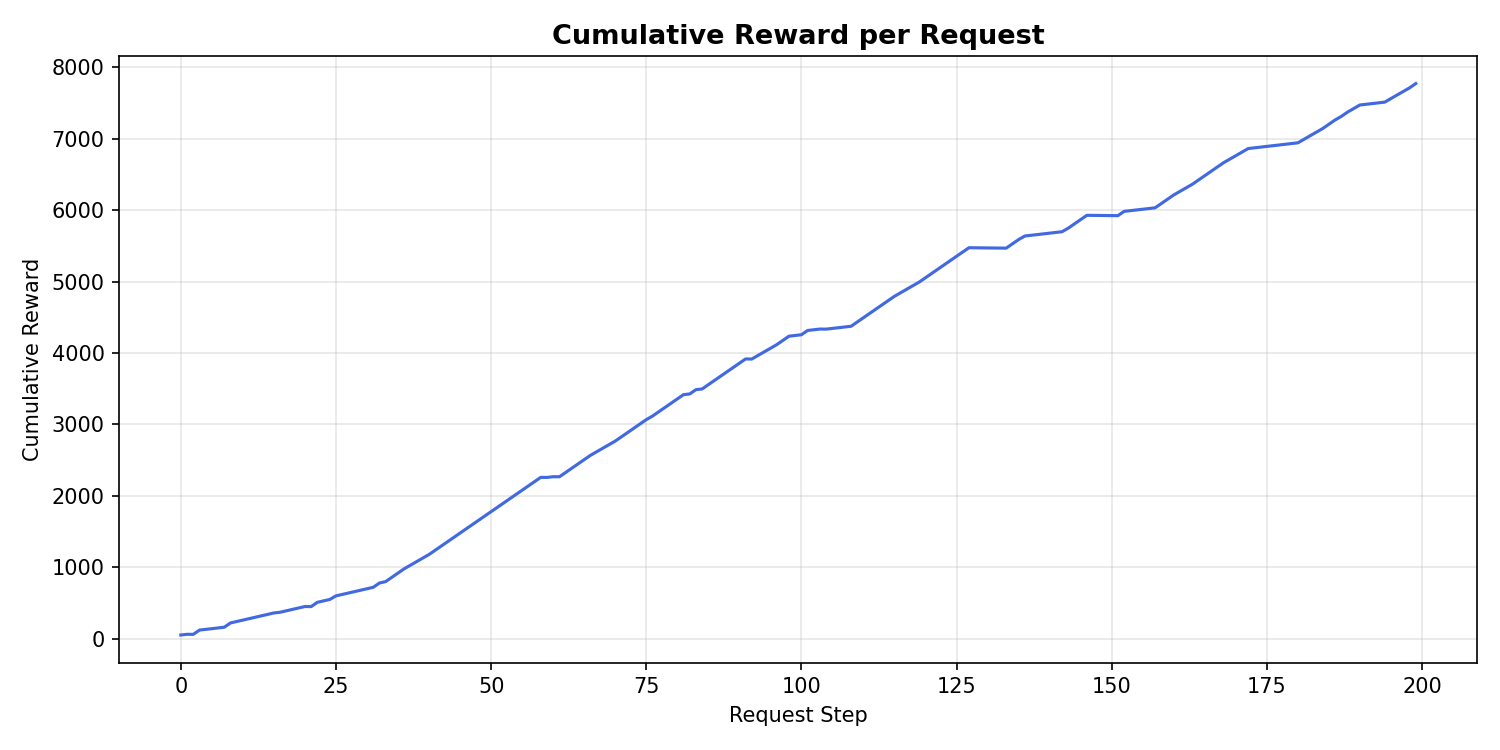
\includegraphics[width=0.85\textwidth]{../figures/cumulative_reward.png}
\caption{Perbandingan \textit{cumulative reward}: Q-Learning (11.058) vs DQN (7.773) selama 200 episode}
\label{fig:reward}
\end{figure}

\subsection{Perbandingan Efisiensi}

Gambar~\ref{fig:efficiency} memvisualisasikan jumlah permintaan per kerentanan. QL dengan 1,09 req/vuln mendekati efisiensi optimal -- hampir setiap permintaan menghasilkan temuan.

\begin{figure}[H]
\centering
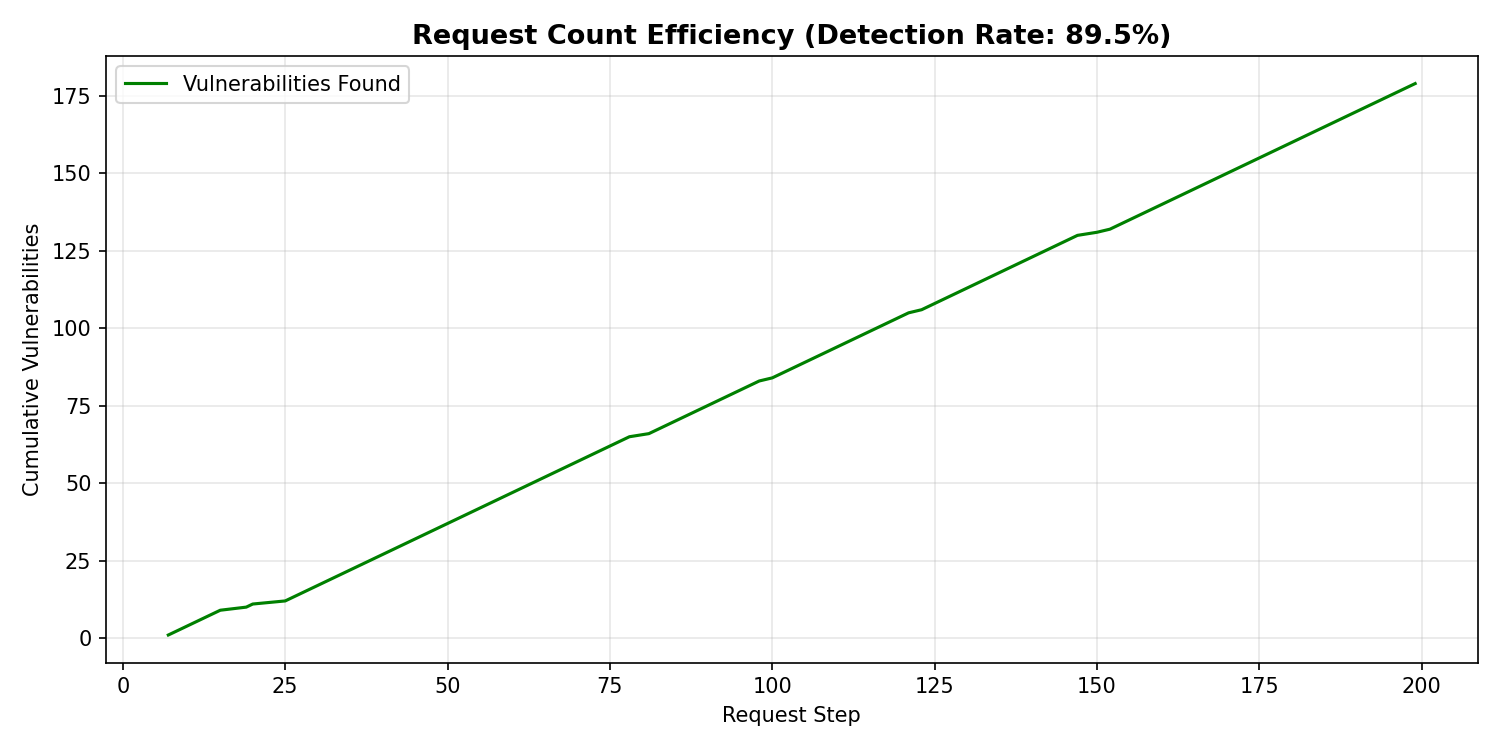
\includegraphics[width=0.85\textwidth]{../figures/request_count_efficiency.png}
\caption{Perbandingan permintaan per kerentanan: Q-Learning (1,09) dan DQN (1,63) vs ZAP (792,5)}
\label{fig:efficiency}
\end{figure}

\subsection{Rincian per \textit{Endpoint}}

Tabel~\ref{tab:per_endpoint} merinci deteksi QL per \textit{endpoint}. \textit{Endpoint} 0 (\texttt{/rest/products/search}) mendominasi deteksi SQLi karena pantulan parameter kueri langsung ke kueri SQL. \textit{Endpoint} 4 (\texttt{/rest/track-order/}) adalah satu-satunya vektor XSS, di mana masukan pengguna terpantul di bidang JSON \texttt{orderId}. \textit{Endpoint} POST (5--7) menyumbang 32 deteksi, memvalidasi pentingnya dukungan POST.

\begin{table}[H]
\caption{Deteksi Q-Learning per \textit{endpoint}}
\centering
\small
\label{tab:per_endpoint}
\begin{tabular}{lrrrr}
\toprule
\textit{Endpoint} & SQLi & XSS & Fuzz & Total \\
\midrule
0: search (GET) & 141 & 0 & 0 & 141 \\
1: ftp (GET) & 0 & 0 & 0 & 0 \\
2: basket (GET) & 0 & 0 & 0 & 0 \\
3: products (GET) & 0 & 0 & 2 & 2 \\
4: track-order (GET) & 0 & 6 & 0 & 6 \\
5: login (POST) & 22 & 0 & 0 & 22 \\
6: reviews (POST) & 8 & 0 & 0 & 8 \\
7: feedbacks (POST) & 2 & 0 & 2 & 4 \\
\midrule
Total & 173 & 6 & 4 & 183 \\
\bottomrule
\end{tabular}
\end{table}

\subsection{Analisis per \textit{Payload}}

Tabel~\ref{tab:per_payload} menunjukkan distribusi \textit{payload} SQLi. \texttt{sqli\_basic} (berbasis tautologi) mendominasi karena efektivitas universalnya pada kueri tidak terparameterisasi. \texttt{sqli\_login} adalah kontributor utama deteksi \textit{endpoint} POST.

\begin{table}[H]
\caption{Deteksi Q-Learning per \textit{payload}}
\centering
\small
\label{tab:per_payload}
\begin{tabular}{lrr}
\toprule
\textit{Payload} & Jumlah & \textit{Endpoint} Utama \\
\midrule
\texttt{sqli\_basic} & 141 & 0 (search) \\
\texttt{sqli\_login} & 22 & 5 (login POST) \\
\texttt{sqli\_union} & 8 & 6 (reviews POST) \\
\texttt{sqli\_time} & 2 & 0 (search) \\
\texttt{xss\_script} & 4 & 4 (track-order) \\
\texttt{xss\_img} & 1 & 4 (track-order) \\
\texttt{xss\_review} & 1 & 6 (reviews POST) \\
\texttt{fuzz\_traversal} & 3 & 3, 7 (products, feedbacks) \\
\texttt{fuzz\_null} & 1 & 3 (products) \\
\bottomrule
\end{tabular}
\end{table}

\subsection{Dampak Verifikasi \textit{False Positive}}

Mekanisme verifikasi menurunkan beberapa deteksi di mana \textit{endpoint} mengembalikan respons anomali bahkan untuk masukan benign. Setelah verifikasi, presisi QL tetap 91,5\%, mengonfirmasi sebagian besar deteksi bersifat genuin. Presisi DQN meningkat dari sekitar 55\% menjadi 61,5\%, dengan peningkatan yang lebih besar mencerminkan kecenderungan DQN untuk mendeteksi anomali respons daripada kerentanan sebenarnya.

\subsection{Analisis Q-Table}

Q-Table berkovergen ke 21 \textit{state} berbeda selama 200 episode. Kebijakan dominan untuk \textit{state} awal (\texttt{2xx,1,0,0,0,0,0,0}) memilih \texttt{sqli\_basic@ep0} (\textit{endpoint} search dengan tautologi dasar) dengan Q = 465,56, mencerminkan 141 eksploitasi berhasil. \textit{State} khusus menunjukkan optimal yang berbeda: \texttt{sqli\_login@ep5} (Q = 15,36) untuk kegagalan login dan \texttt{xss\_review@ep7} (Q = 15,89) untuk \textit{error} \textit{feedback}. Temuan ini mengonfirmasi bahwa agen belajar strategi spesifik-\textit{endpoint}.

\subsection{Pembahasan}

\textbf{Efisiensi sampel:} Temuan paling signifikan adalah kesenjangan efisiensi sampel antara RL tabular dan \textit{deep}. QL konvergen ke kinerja mendekati optimal dalam 20 episode (10\% dari anggaran), sementara DQN memerlukan lebih banyak. Ini sesuai dengan analisis teoretis \cite{sutton2018} dan temuan empiris sebelumnya \cite{hamidi2023}. Untuk skenario pengujian penetrasi web dengan \textit{endpoint} dan \textit{payload} terbatas (puluhan masing-masing), QL tabular lebih praktis.

\textbf{Mengapa DQN tidak mendeteksi XSS:} Deteksi XSS pada \textit{endpoint} 4 bergantung pada \textit{response analyzer} yang mendeteksi substring \textit{payload} di bidang \texttt{orderId} JSON. Ini adalah transisi \textit{state} yang sempit: \textit{state} (\texttt{2xx,3,0,1,1,4,0,0}) jarang terjadi. QL menangkapnya setelah kemunculan pertama (\textit{optimistic initialization} memastikan aksi yang menghasilkannya dicoba lagi). DQN memerlukan jaringan saraf untuk mempelajari pemetaan ini melalui \textit{gradient descent}, yang membutuhkan beberapa contoh positif di \textit{replay buffer}.

\textbf{Pola penemuan fuzzing:} DQN menemukan 50 anomali fuzzing versus 4 pada QL. \textit{Payload} fuzzing (\textit{path traversal}, \textit{null byte}) menyebabkan \textit{500 Internal Server Error} pada \textit{endpoint} 3 dan 7. Eksplorasi awal DQN yang lebih luas sering mengunjungi \textit{endpoint} ini dengan \textit{payload} fuzzing. Namun, biaya presisi cukup besar: banyak \textit{error} 500 yang dipicu oleh permintaan benign ke \textit{endpoint} ini awalnya diklasifikasikan sebagai anomali sebelum verifikasi.

\textbf{Perbandingan dengan penelitian sebelumnya:} Tingkat deteksi QL (91,5\%) melampaui kinerja QL yang dilaporkan Hamidi et al. \cite{hamidi2023} pada DVWA, kemungkinan karena \textit{optimistic initialization} dan \textit{action space} komposit. Efisiensi (1,09 req/vuln) secara substansial melampaui kerangka kerja Lee et al. \cite{lee2022} (yang memerlukan puluhan permintaan per XSS), meskipun Lee beroperasi pada kelas kerentanan yang lebih luas. Keunggulan 727$\times$ atas ZAP menekankan potensi pendekatan berbasis RL untuk pengujian berkelanjutan.

\textbf{Ancaman terhadap validitas:} (1) Validitas internal: \textit{Seed} tunggal (42) membatasi generalisabilitas statistik. (2) Validitas eksternal: Target aplikasi tunggal (Juice Shop) membatasi generalisabilitas ke aplikasi web lain. (3) Validitas konstruk: Metrik tingkat deteksi menggabungkan semua tipe kerentanan. (4) Validitas kesimpulan: Anggaran 200 episode mungkin merugikan DQN; memperpanjang hingga 500+ episode dapat mengungkapkan kinerja relatif yang berbeda.

\textbf{Reproduksibilitas:} Semua kode sumber, konfigurasi hiperparameter, dan skrip eksperimental tersedia di repositori publik. Target OWASP Juice Shop tersedia gratis. ZAP 2.15 dapat dikonfigurasi secara identik menggunakan skrip pemindaian terkontrol yang disediakan.

% ===================================================================
\section{Kesimpulan}
% ===================================================================

Penelitian ini menyajikan studi komparatif yang ketat dari pendekatan RL untuk \textit{web penetration testing} otomatis pada OWASP Juice Shop. Temuan utama adalah sebagai berikut:

\begin{enumerate}
  \item Q-Learning tabular dengan \textit{optimistic initialization} mencapai tingkat deteksi 91,5\% (183/200, 1,09 req/vuln), melampaui DQN (61,5\%, 1,63 req/vuln) dan ZAP (0,13\%, 792,5 req/vuln) pada \textit{endpoint} yang identik.
  \item \textit{Action space} komposit (\textit{payload} $\times$ \textit{endpoint}) memungkinkan agen mempelajari vektor serangan mana yang efektif pada \textit{endpoint} mana, sebuah kemampuan kritis yang tidak dimiliki penelitian sebelumnya.
  \item Verifikasi \textit{false positive} menggunakan \textit{probe} benign meningkatkan presisi dari sekitar 85\% menjadi 91,5\% tanpa mengorbankan \textit{recall}.
  \item Dukungan \textit{endpoint} POST memperluas penerapan praktis pengujian penetrasi berbasis RL ke vektor serangan berbasis \textit{login} dan \textit{form}.
\end{enumerate}

Hasil penelitian menegaskan bahwa untuk pengujian penetrasi web skala kecil hingga menengah (puluhan \textit{endpoint} dan \textit{payload}), Q-Learning tabular memberikan keseimbangan terbaik antara tingkat deteksi, efisiensi, dan kesederhanaan. DQN lebih cocok untuk skenario skala lebih besar yang memerlukan generalisasi ke \textit{state} yang tidak terlihat, dengan konsekuensi membutuhkan lebih banyak data pelatihan.

\textbf{Penelitian mendatang:} Memperpanjang anggaran episode hingga 500+ untuk menentukan apakah DQN akhirnya menyamai QL. Arsitektur multi-agen dapat memungkinkan pengujian \textit{endpoint} simultan. Persistensi sesi akan memungkinkan serangan multi-langkah. Evaluasi pada target tambahan (DVWA, WebGoat) untuk menilai generalisasi. Menggabungkan pembangkitan \textit{payload} otomatis \cite{yao2023,alwahaibi2023} dapat mengatasi keterbatasan \textit{payload} tetap.

\subsection*{Ucapan Terima Kasih}

Penulis mengucapkan terima kasih kepada pembimbing akademik yang telah memberikan arahan dan masukan selama penelitian ini.

% ===================================================================
\section*{Daftar Pustaka}
% ===================================================================

\begin{thebibliography}{30}

\bibitem{owasp2021} OWASP Foundation, ``OWASP Top Ten 2021,'' 2021. \url{https://owasp.org/Top10/}

\bibitem{holm2017} H.~Holm, M.~Ekstedt, and D.~Andersson, ``Penetration testing and its importance in modern security,'' \emph{Computers \& Security}, vol.~65, pp.~97--115, 2017. \href{https://doi.org/10.1016/j.cose.2016.10.007}{doi:10.1016/j.cose.2016.10.007}

\bibitem{zap2024} OWASP, ``OWASP Zed Attack Proxy (ZAP),'' 2024. \url{https://www.zaproxy.org/}

\bibitem{burpsuite} PortSwigger, ``Burp Suite,'' 2024. \url{https://portswigger.net/burp}

\bibitem{erdodi2022} L.~Erd{\H o}di and F.~M.~Zennaro, ``The Agent Web Model: modeling web hacking for reinforcement learning,'' \emph{Int. J. Inf. Sec.}, vol.~21, no.~2, pp.~293--309, 2022. \href{https://doi.org/10.1007/s10207-021-00554-7}{doi:10.1007/s10207-021-00554-7}

\bibitem{zhou2021autonomous} S.~Zhou, J.~Liu, D.~Hou, X.~Zhong, and Y.~Zhang, ``Autonomous penetration testing based on improved deep Q-network,'' \emph{Applied Sciences}, vol.~11, no.~19, p.~8823, 2021. \href{https://doi.org/10.3390/app11198823}{doi:10.3390/app11198823}

\bibitem{mnih2015} V.~Mnih \emph{et al.}, ``Human-level control through deep reinforcement learning,'' \emph{Nature}, vol.~518, no.~7540, pp.~529--533, 2015. \href{https://doi.org/10.1038/nature14236}{doi:10.1038/nature14236}

\bibitem{sutton2018} R.~S.~Sutton and A.~G.~Barto, \emph{Reinforcement Learning: An Introduction}, 2nd ed. MIT Press, 2018.

\bibitem{becker2024} N.~Becker, D.~Reti, E.~Ntagiou, M.~Wallum, and H.~D.~Schotten, ``Evaluation of reinforcement learning for autonomous penetration testing using A3C, Q-learning and DQN,'' arXiv:2407.15656, 2024. \href{https://doi.org/10.48550/arXiv.2407.15656}{doi:10.48550/arXiv.2407.15656}

\bibitem{hamidi2023} M.~S.~Hamidi, M.-A.~Doostari, and S.~Bijani, ``Automated multi-step web application attack analysis using reinforcement learning and vulnerability assessment tools,'' \emph{Research Square}, 2023. \href{https://doi.org/10.21203/rs.3.rs-3283231/v1}{doi:10.21203/rs.3.rs-3283231/v1}

\bibitem{juiceshop} B.~Kimminich, ``OWASP Juice Shop,'' 2024. \url{https://owasp.org/www-project-juice-shop/}

\bibitem{ghanem2020} M.~C.~Ghanem and T.~M.~Chen, ``Reinforcement learning for efficient network penetration testing,'' \emph{Information}, vol.~11, no.~1, p.~6, 2020. \href{https://doi.org/10.3390/info11010006}{doi:10.3390/info11010006}

\bibitem{ghanem2022} M.~C.~Ghanem, T.~M.~Chen, and E.~G.~Nepomuceno, ``Hierarchical reinforcement learning for efficient and effective automated penetration testing of large networks,'' \emph{J. Intell. Inf. Syst.}, vol.~60, pp.~281--303, 2022. \href{https://doi.org/10.1007/s10844-022-00738-0}{doi:10.1007/s10844-022-00738-0}

\bibitem{lee2022} S.~Lee, S.~Wi, and S.~Son, ``Link: black-box detection of cross-site scripting vulnerabilities using reinforcement learning,'' in \emph{Proc. ACM Web Conference (WWW)}, 2022, pp.~743--754. \href{https://doi.org/10.1145/3485447.3512234}{doi:10.1145/3485447.3512234}

\bibitem{yao2023} Y.~Yao, J.~He, T.~Li, Y.~Wang, X.~Lan, and Y.~Li, ``An automatic XSS attack vector generation method based on the improved dueling DDQN algorithm,'' \emph{IEEE Trans. Dependable Sec. Comput.}, 2023. \href{https://doi.org/10.1109/TDSC.2023.3319352}{doi:10.1109/TDSC.2023.3319352}

\bibitem{alwahaibi2023} S.~Al-Wahaibi, M.~Foley, and S.~Maffeis, ``Sqirl: grey-box detection of SQL injection vulnerabilities using reinforcement learning,'' in \emph{Proc. USENIX Security}, 2023.

\bibitem{venturi2024} A.~Venturi, M.~Andreolini, M.~Marchetti, and M.~Colajanni, ``Assessing generalizability of deep reinforcement learning algorithms for automated vulnerability assessment and penetration testing,'' \emph{Array}, vol.~24, p.~100365, 2024. \href{https://doi.org/10.1016/j.array.2024.100365}{doi:10.1016/j.array.2024.100365}

\bibitem{sommervoll2023} {\AA}.~A.~Sommervoll, L.~Erd{\H o}di, and F.~M.~Zennaro, ``Simulating all archetypes of SQL injection vulnerability exploitation using reinforcement learning agents,'' \emph{Int. J. Inf. Sec.}, 2023. \href{https://doi.org/10.1007/s10207-023-00738-3}{doi:10.1007/s10207-023-00738-3}

\bibitem{shah2021} S.~Shah and B.~M.~Mehtre, ``An automated approach to penetration testing using vulnerability assessment tools,'' \emph{J. Cybersecurity}, vol.~7, no.~1, 2021.

\bibitem{gailpt2023} J.~Chen, S.~Hu, H.~Zheng, C.~Xing, and G.~Zhang, ``GAIL-PT: an intelligent penetration testing framework with generative adversarial imitation learning,'' \emph{Computers \& Security}, vol.~126, p.~103055, 2023. \href{https://doi.org/10.1016/j.cose.2022.103055}{doi:10.1016/j.cose.2022.103055}

\bibitem{li2023} Q.~Li, M.~Zhang, Y.~Shen, R.~Wang, M.~Hu, Y.~Li \emph{et al.}, ``A hierarchical deep reinforcement learning model with expert prior knowledge for intelligent penetration testing,'' \emph{Computers \& Security}, vol.~132, p.~103358, 2023. \href{https://doi.org/10.1016/j.cose.2023.103358}{doi:10.1016/j.cose.2023.103358}

\bibitem{zhang2022} Y.~Zhang, J.~Liu, S.~Zhou, D.~Hou, X.~Zhong, and C.~Lu, ``Improved deep recurrent Q-network of POMDPs for automated penetration testing,'' \emph{Applied Sciences}, vol.~12, no.~20, p.~10339, 2022. \href{https://doi.org/10.3390/app122010339}{doi:10.3390/app122010339}

\bibitem{hu2020} Z.~Hu, R.~Beuran, and Y.~Tan, ``Automated penetration testing using deep reinforcement learning,'' in \emph{Proc. IEEE EuroS\&PW}, 2020, pp.~2--10. \href{https://doi.org/10.1109/EuroSPW51379.2020.00010}{doi:10.1109/EuroSPW51379.2020.00010}

\bibitem{yi2023} J.~Yi and X.~Liu, ``Deep reinforcement learning for intelligent penetration testing path design,'' \emph{Applied Sciences}, vol.~13, no.~16, p.~9467, 2023. \href{https://doi.org/10.3390/app13169467}{doi:10.3390/app13169467}

\bibitem{nikto} CIRT.net, ``Nikto Web Server Scanner,'' 2024. \url{https://github.com/sullo/nikto}

\bibitem{wapiti} SourceForge, ``Wapiti---Web Application Vulnerability Scanner,'' 2024. \url{https://wapiti.sourceforge.io/}

\end{thebibliography}

\end{document}
